

\documentclass[12pt,a4paper]{article}\usepackage[]{graphicx}\usepackage[]{color}
%% maxwidth is the original width if it is less than linewidth
%% otherwise use linewidth (to make sure the graphics do not exceed the margin)
\makeatletter
\def\maxwidth{ %
  \ifdim\Gin@nat@width>\linewidth
    \linewidth
  \else
    \Gin@nat@width
  \fi
}
\makeatother

\definecolor{fgcolor}{rgb}{0.345, 0.345, 0.345}
\newcommand{\hlnum}[1]{\textcolor[rgb]{0.686,0.059,0.569}{#1}}%
\newcommand{\hlstr}[1]{\textcolor[rgb]{0.192,0.494,0.8}{#1}}%
\newcommand{\hlcom}[1]{\textcolor[rgb]{0.678,0.584,0.686}{\textit{#1}}}%
\newcommand{\hlopt}[1]{\textcolor[rgb]{0,0,0}{#1}}%
\newcommand{\hlstd}[1]{\textcolor[rgb]{0.345,0.345,0.345}{#1}}%
\newcommand{\hlkwa}[1]{\textcolor[rgb]{0.161,0.373,0.58}{\textbf{#1}}}%
\newcommand{\hlkwb}[1]{\textcolor[rgb]{0.69,0.353,0.396}{#1}}%
\newcommand{\hlkwc}[1]{\textcolor[rgb]{0.333,0.667,0.333}{#1}}%
\newcommand{\hlkwd}[1]{\textcolor[rgb]{0.737,0.353,0.396}{\textbf{#1}}}%
\let\hlipl\hlkwb

\usepackage{framed}
\makeatletter
\newenvironment{kframe}{%
 \def\at@end@of@kframe{}%
 \ifinner\ifhmode%
  \def\at@end@of@kframe{\end{minipage}}%
  \begin{minipage}{\columnwidth}%
 \fi\fi%
 \def\FrameCommand##1{\hskip\@totalleftmargin \hskip-\fboxsep
 \colorbox{shadecolor}{##1}\hskip-\fboxsep
     % There is no \\@totalrightmargin, so:
     \hskip-\linewidth \hskip-\@totalleftmargin \hskip\columnwidth}%
 \MakeFramed {\advance\hsize-\width
   \@totalleftmargin\z@ \linewidth\hsize
   \@setminipage}}%
 {\par\unskip\endMakeFramed%
 \at@end@of@kframe}
\makeatother

\definecolor{shadecolor}{rgb}{.97, .97, .97}
\definecolor{messagecolor}{rgb}{0, 0, 0}
\definecolor{warningcolor}{rgb}{1, 0, 1}
\definecolor{errorcolor}{rgb}{1, 0, 0}
\newenvironment{knitrout}{}{} % an empty environment to be redefined in TeX

\usepackage{alltt}
\usepackage{amsmath}
\usepackage{enumerate}
\usepackage[cm]{fullpage}
\usepackage{graphicx}
\IfFileExists{upquote.sty}{\usepackage{upquote}}{}
\begin{document}
\setlength\parindent{0cm}
%\setlength{\oddsidemargin}{0.25cm}
%\setlength{\evensidemargin}{0.25cm}
\title{\Large{\textbf{Introduction to \texttt{R}}}\\
\textit{Answers to Session 6 exercises}}
\author{Statistical Consulting Center}
\date{15 November, 2016}
\maketitle
 

\begin{enumerate}
\item Plot the mean nerdy score for each gender (with $\pm$1.96$\times$SE bars), as shown in Figure \ref{fig:stder1}. 
\begin{figure}[h]   
 \centering
\begin{knitrout}
\definecolor{shadecolor}{rgb}{0.969, 0.969, 0.969}\color{fgcolor}\begin{kframe}
\begin{alltt}
\hlstd{g.m} \hlkwb{<-} \hlkwd{with}\hlstd{(sports.df,} \hlkwd{tapply}\hlstd{(nerdy.sc, gender, mean,} \hlkwc{na.rm} \hlstd{= T))}
\hlstd{g.sd} \hlkwb{<-} \hlkwd{with}\hlstd{(sports.df,} \hlkwd{tapply}\hlstd{(nerdy.sc, gender, sd,} \hlkwc{na.rm} \hlstd{= T))}
\hlstd{g.n} \hlkwb{<-} \hlkwd{with}\hlstd{(sports.df,} \hlkwd{tapply}\hlstd{(nerdy.sc, gender,} \hlkwa{function}\hlstd{(}\hlkwc{x}\hlstd{)}\hlkwd{sum}\hlstd{(}\hlopt{!}\hlkwd{is.na}\hlstd{(x))))}
\hlstd{g.stder} \hlkwb{<-} \hlstd{g.sd}\hlopt{/}\hlkwd{sqrt}\hlstd{(g.n)}
\hlstd{g.upper} \hlkwb{<-}\hlstd{g.m} \hlopt{+} \hlnum{1.96}\hlopt{*}\hlstd{g.stder}
\hlstd{g.lower} \hlkwb{<-}\hlstd{g.m} \hlopt{-} \hlnum{1.96}\hlopt{*}\hlstd{g.stder}
\hlkwd{plot}\hlstd{(g.m,} \hlkwc{xlim} \hlstd{=} \hlkwd{c}\hlstd{(}\hlnum{0}\hlstd{,} \hlnum{3}\hlstd{),} \hlkwc{ylim} \hlstd{=} \hlkwd{range}\hlstd{(}\hlkwd{c}\hlstd{(g.upper, g.lower)),} \hlkwc{xlab} \hlstd{=} \hlstr{"Gender"}\hlstd{,}
     \hlkwc{ylab} \hlstd{=} \hlstr{"Mean nerdy score"}\hlstd{,} \hlkwc{axes} \hlstd{= F)}
\hlkwd{arrows}\hlstd{(}\hlnum{1}\hlopt{:}\hlnum{2}\hlstd{, g.upper,} \hlnum{1}\hlopt{:}\hlnum{2}\hlstd{, g.lower,} \hlkwc{length} \hlstd{=} \hlnum{0.1}\hlstd{,} \hlkwc{code} \hlstd{=} \hlnum{3}\hlstd{,} \hlkwc{angle} \hlstd{=} \hlnum{90}\hlstd{)}
\hlkwd{axis}\hlstd{(}\hlnum{2}\hlstd{)}
\hlkwd{axis}\hlstd{(}\hlnum{1}\hlstd{,} \hlkwc{at}\hlstd{=}\hlnum{1}\hlopt{:}\hlnum{2}\hlstd{,} \hlkwc{labels} \hlstd{=} \hlkwd{names}\hlstd{(g.m))}
\hlkwd{box}\hlstd{()}
\end{alltt}
\end{kframe}
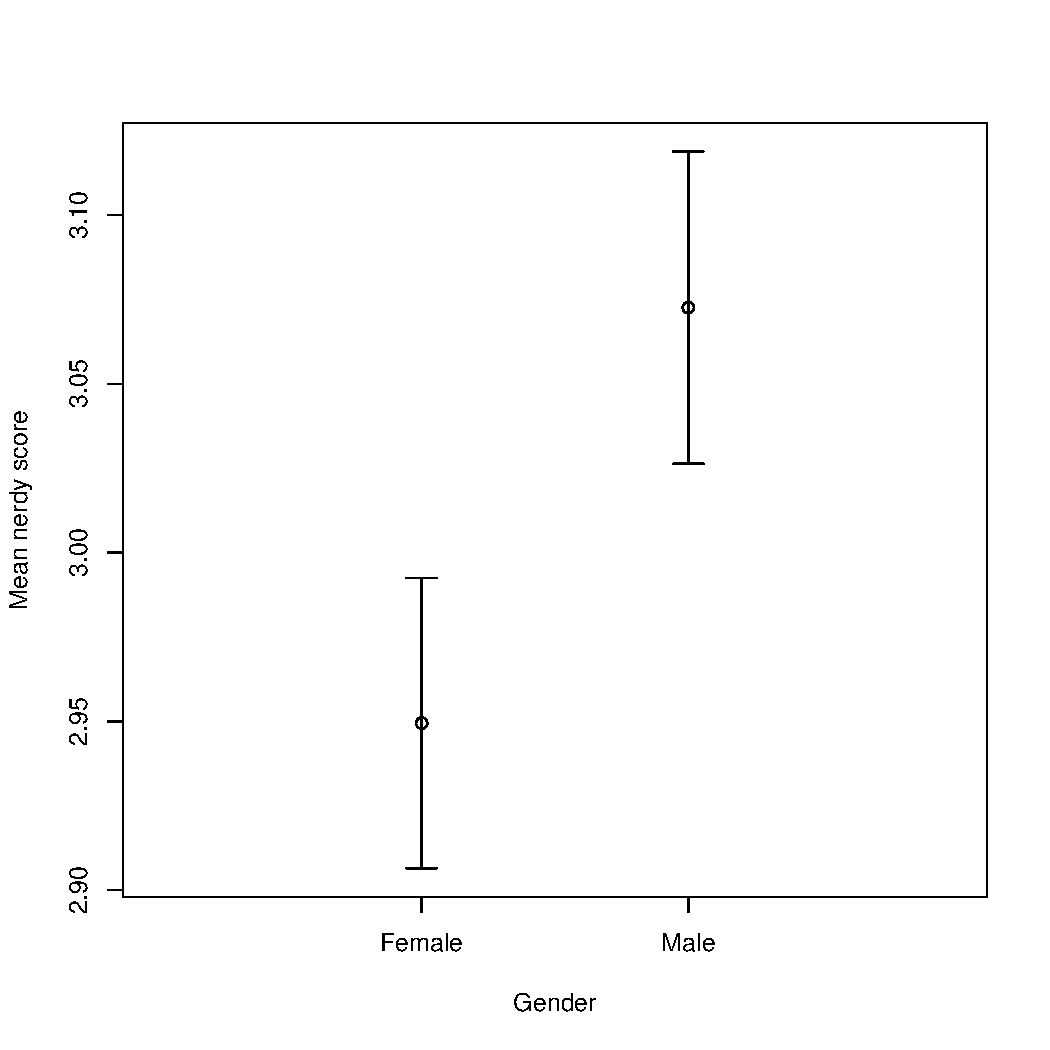
\includegraphics[width=0.5\textwidth]{figure/stder1-1} 

\end{knitrout}
\caption{First plot with standard error bars}
  \label{fig:stder1}
\end{figure}
\newpage
\item Now reproduce Figure \ref{fig:stder2}. The graph should have:
\begin{itemize}
\item for Males: \textcolor{blue}{blue} solid circles (representing the mean) and $\pm$1.96$\times$SE bars (representing the lower and upper 95\% confidence limits).
\item for Females: \textcolor{red}{red} solid circles (representing the mean) and $\pm$1.96$\times$SE bars (representing the lower and upper 95\% confidence limits).
\end{itemize}
\begin{figure}[h]   
 \centering
\begin{knitrout}
\definecolor{shadecolor}{rgb}{0.969, 0.969, 0.969}\color{fgcolor}\begin{kframe}
\begin{alltt}
\hlstd{ga.m} \hlkwb{<-} \hlkwd{with}\hlstd{(sports.df,} \hlkwd{tapply}\hlstd{(nerdy.sc,} \hlkwd{list}\hlstd{(gender, age.group), mean,} \hlkwc{na.rm} \hlstd{=} \hlnum{TRUE}\hlstd{))}
\hlstd{ga.sd} \hlkwb{<-} \hlkwd{with}\hlstd{(sports.df,} \hlkwd{tapply}\hlstd{(nerdy.sc,} \hlkwd{list}\hlstd{(gender, age.group), sd,} \hlkwc{na.rm} \hlstd{=} \hlnum{TRUE}\hlstd{))}
\hlstd{ga.n} \hlkwb{<-} \hlkwd{with}\hlstd{(sports.df,} \hlkwd{tapply}\hlstd{(nerdy.sc,} \hlkwd{list}\hlstd{(gender, age.group),}
                               \hlkwa{function}\hlstd{(}\hlkwc{x}\hlstd{)}\hlkwd{sum}\hlstd{(}\hlopt{!}\hlkwd{is.na}\hlstd{(x))))}
\hlstd{ga.stder} \hlkwb{<-} \hlstd{ga.sd}\hlopt{/}\hlkwd{sqrt}\hlstd{(ga.n)}
\hlstd{ga.upper} \hlkwb{<-}\hlstd{ga.m} \hlopt{+} \hlnum{1.96}\hlopt{*}\hlstd{ga.stder}
\hlstd{ga.lower} \hlkwb{<-}\hlstd{ga.m} \hlopt{-} \hlnum{1.96}\hlopt{*}\hlstd{ga.stder}
\hlkwd{plot}\hlstd{(}\hlkwd{c}\hlstd{(}\hlnum{1}\hlstd{,} \hlnum{3}\hlstd{,} \hlnum{5}\hlstd{), ga.m[}\hlnum{1}\hlstd{, ],} \hlkwc{xlim} \hlstd{=} \hlkwd{c}\hlstd{(}\hlnum{0}\hlstd{,} \hlnum{6.5}\hlstd{),} \hlkwc{ylim} \hlstd{=} \hlkwd{range}\hlstd{(}\hlkwd{c}\hlstd{(ga.upper, ga.lower)),}
     \hlkwc{xlab} \hlstd{=} \hlstr{"Age Group"}\hlstd{,} \hlkwc{ylab} \hlstd{=} \hlstr{"Mean nerdy score"}\hlstd{,} \hlkwc{axes} \hlstd{= F,} \hlkwc{col} \hlstd{=} \hlnum{2}\hlstd{,} \hlkwc{pch} \hlstd{=} \hlnum{19}\hlstd{)}
\hlkwd{arrows}\hlstd{(}\hlkwd{c}\hlstd{(}\hlnum{1}\hlstd{,} \hlnum{3}\hlstd{,} \hlnum{5}\hlstd{), ga.upper[}\hlnum{1}\hlstd{, ],} \hlkwd{c}\hlstd{(}\hlnum{1}\hlstd{,} \hlnum{3}\hlstd{,} \hlnum{5}\hlstd{), ga.lower[}\hlnum{1}\hlstd{, ],}
       \hlkwc{length} \hlstd{=} \hlnum{0.1}\hlstd{,} \hlkwc{code} \hlstd{=} \hlnum{3}\hlstd{,} \hlkwc{angle} \hlstd{=} \hlnum{90}\hlstd{,} \hlkwc{col} \hlstd{=} \hlnum{2}\hlstd{)}
\hlkwd{points}\hlstd{(}\hlkwd{c}\hlstd{(}\hlnum{1.5}\hlstd{,} \hlnum{3.5}\hlstd{,} \hlnum{5.5}\hlstd{), ga.m[}\hlnum{2}\hlstd{, ],} \hlkwc{col} \hlstd{=} \hlnum{4}\hlstd{,} \hlkwc{pch} \hlstd{=} \hlnum{19}\hlstd{)}
\hlkwd{arrows}\hlstd{(}\hlkwd{c}\hlstd{(}\hlnum{1.5}\hlstd{,} \hlnum{3.5}\hlstd{,} \hlnum{5.5}\hlstd{), ga.upper[}\hlnum{2}\hlstd{, ],} \hlkwd{c}\hlstd{(}\hlnum{1.5}\hlstd{,} \hlnum{3.5}\hlstd{,} \hlnum{5.5}\hlstd{), ga.lower[}\hlnum{2}\hlstd{, ],}
       \hlkwc{length} \hlstd{=} \hlnum{0.1}\hlstd{,} \hlkwc{code} \hlstd{=} \hlnum{3}\hlstd{,} \hlkwc{angle} \hlstd{=} \hlnum{90}\hlstd{,} \hlkwc{col} \hlstd{=} \hlnum{4}\hlstd{)}
\hlkwd{axis}\hlstd{(}\hlnum{2}\hlstd{)}
\hlkwd{axis}\hlstd{(}\hlnum{1}\hlstd{,} \hlkwc{at}\hlstd{=}\hlkwd{c}\hlstd{(}\hlnum{1.25}\hlstd{,} \hlnum{3.25}\hlstd{,} \hlnum{5.25}\hlstd{),} \hlkwc{labels} \hlstd{=} \hlkwd{colnames}\hlstd{(ga.m))}
\hlkwd{box}\hlstd{()}
\hlkwd{legend}\hlstd{(}\hlstr{"topright"}\hlstd{,} \hlkwc{pch} \hlstd{=} \hlnum{19}\hlstd{,} \hlkwc{lty} \hlstd{=} \hlnum{1}\hlstd{,} \hlkwc{col} \hlstd{=} \hlkwd{c}\hlstd{(}\hlnum{2}\hlstd{,} \hlnum{4}\hlstd{),}
       \hlkwc{legend} \hlstd{=} \hlkwd{row.names}\hlstd{(ga.m),} \hlkwc{bty} \hlstd{=} \hlstr{"n"}\hlstd{)}
\end{alltt}
\end{kframe}
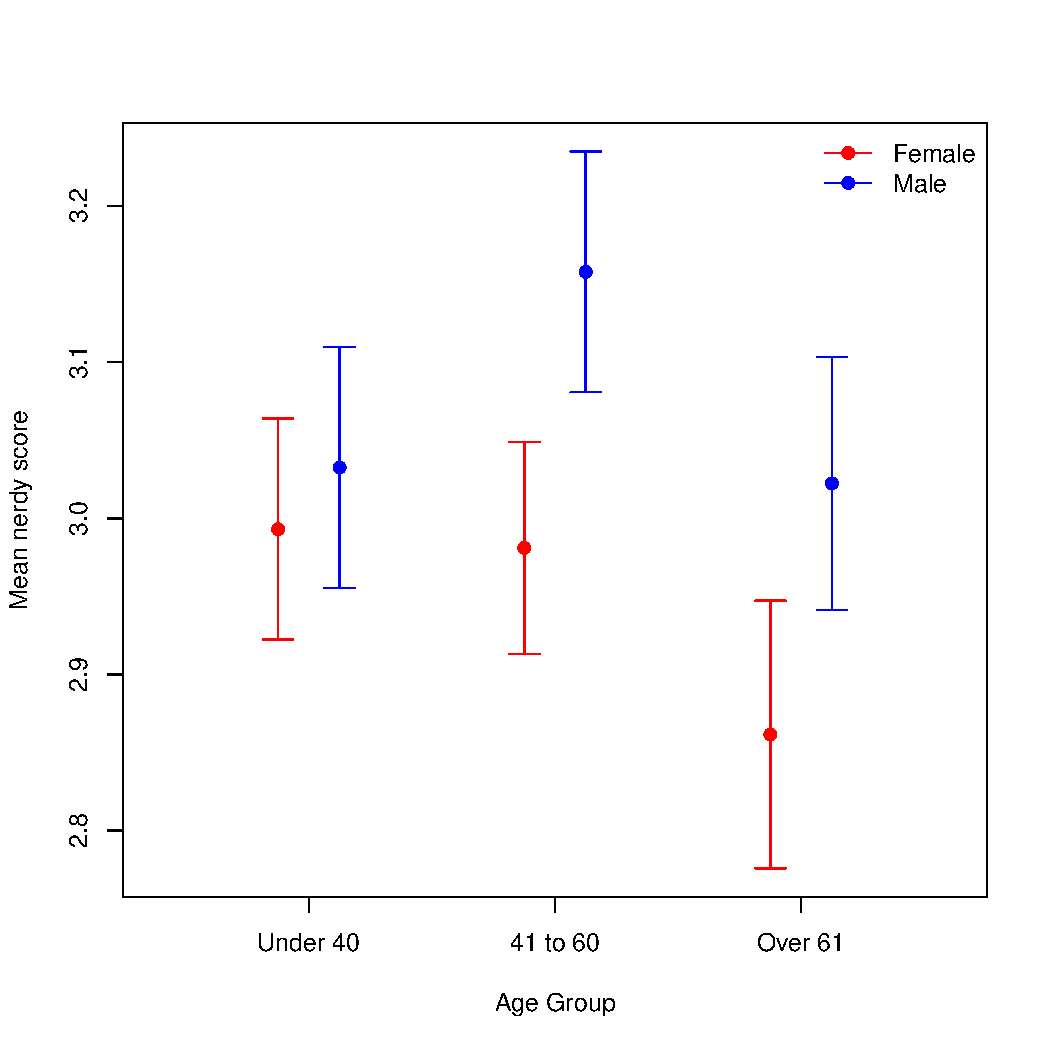
\includegraphics[width=0.45\textwidth]{figure/stder2-1} 

\end{knitrout}
\caption{Second plot with standard error bars}
  \label{fig:stder2}
\end{figure}
\end{enumerate}
\end{document}
